% $Id: GMAT-Architectural-Specification.tex,v 1.34 2007/12/21 17:00:37 dconway Exp $
\documentclass[letterpaper,10pt]{book}

\usepackage[T1]{fontenc}
\usepackage[latin1]{inputenc}
\usepackage{geometry}
\usepackage{graphics,color}
\usepackage{overcite}
\geometry{letterpaper}

% Used to customize captions
\usepackage[pointedenum]{paralist}

% Enable indexing
\usepackage{makeidx}
\makeindex

%  for showing script lines as they appear in GMAT
\usepackage{verbatim}

% Allows alignment of multiple columns of text
\usepackage{array}

% Enables text wrapping around small tables and figures
\usepackage{float}

% Enables text wrapping around small tables and figures
\usepackage{floatflt}

% Enables side by side figures
\usepackage[countmax]{subfloat}

% Enables line numbering for verbatim text
\usepackage{lineno}

% Some text listing help for script files
\usepackage{listings}
\lstset{frame=single, captionpos=b, language=Matlab, xleftmargin=36pt, xrightmargin=36pt,
basicstyle=\ttfamily, numberstyle=\tiny, numbers=none}

% Use special characters defined by the ams
\usepackage{amsmath}

% Allow rotating figures
\usepackage{lscape}

% Enable verbatiminput so functional script files can be read in directly
\usepackage{fancyvrb}

% Fixes some font sizing problems
\usepackage{fix-cm}

%  for making index, using landscape mode, for multi page tables, supertabular??
% This package is needed to include the tables in the GMATDocuments/common subfolder
\usepackage{longtable, supertabular}

%\usepackage{rotating}  %This breaks the png files in \includegraphics{} calls???

% Used for table organization
\usepackage{tabularx}

%\usepackage[listofnumwidth=5.5em]{subfig}

% Used to customize table and figure list spacings
\usepackage{tocloft}

% Used to customize captions
\usepackage{caption}

% for creating bookmarks in the final pdf file when using dvipdfm
\usepackage[dvipdfm, bookmarks = true, bookmarksopen]{hyperref}

%% Used to build enumerations of the form 1.2.3.4.  etc.
%\usepackage[pointedenum]{paralist}

% If going through postscript to pdf, use the following instead for bookmarks:
%\usepackage[dvips, bookmarks = true, bookmarksopen]{hyperref}

%% Used to build the glossary and acronym definitions
%\usepackage[toc]{glossaries}

% Construct the basic page sizes
\oddsidemargin  0.0in
\evensidemargin 0.0in
\textwidth      6.5in
\headheight     0.25in
\topmargin      0.0in
\textheight=8.5in

% Note that png and jpg extensions are used for graphics
\DeclareGraphicsExtensions{.png,.jpg}

%% The following lines customize spacing on the tables of contents, list of figures, etc.
% More space for figure numbers
\setlength{\cftfignumwidth}{3em}
% Space between elements of the list
%\setlength{\cftbeforefigskip}{0.1cm}
% Space before chapter entries in the TOC
%\setlength{\cftbeforechapskip}{0.2cm}
% Space before parts in the TOC
%\setlength{\cftbeforepartskip}{0.7cm}

%\setlength{\emergencystretch}{6em}
%\pretolerance=10000
%\tolerance=10000

%\define@key{caption}{listofnumwidth}[4em]{\def\sf@numwidth{#1}}


%-------------------------------------------------------------------------------
%------------------------------------New Commands-------------------------------
%-------------------------------------------------------------------------------
\newcommand{\st}[1]{\begin{ttfamily}#1\end{ttfamily}}
\newcommand{\boldst}[1]{\begin{ttfamily}\textbf{#1} \end{ttfamily}}
\newcommand{\br}[0]{$\mathbf{r} $}
\newcommand{\bv}[0]{$\mathbf{v} $}
\newcommand{\ba}[0]{$\mathbf{a} $}
\newcommand{\mbr}[0]{\mathbf{r} }
\newcommand{\mbv}[0]{\mathbf{v} }
\newcommand{\mba}[0]{\mathbf{a} }

%-------------------------------------------------------------------------------
%------------------------------------New Environments---------------------------
%-------------------------------------------------------------------------------

\newenvironment{ScriptType}
  {\noindent \begin{ttfamily}}
   { \end{ttfamily} }

\newenvironment{Script}
 { \vspace{-.15 in} \begin{ttfamily} }
 { \end{ttfamily}\vspace{-.25 in} }

% Turned off the watermark for now because it's annoying in proof mode
% Make the watermark
\usepackage{eso-pic}
\usepackage{color}
\usepackage{type1cm}
%\makeatletter
%  \AddToShipoutPicture{%
%    \setlength{\@tempdimb}{.5\paperwidth}%
%    \setlength{\@tempdimc}{.5\paperheight}%
%    \setlength{\unitlength}{1pt}%
%    \put(\strip@pt\@tempdimb,\strip@pt\@tempdimc){%
%      \makebox(0,0){\rotatebox{45}{\textcolor[gray]{0.75}{\fontsize{2cm}{2cm}\selectfont{Draft:
%Work in Progress}}}}
%    }
%} \makeatother

% Disabled for intermediate versions -- TURN ON FOR RELEASE VERSIONS
%\makeatletter
%  \AddToShipoutPicture{%
%    \setlength{\@tempdimb}{.5\paperwidth}%
%    \setlength{\@tempdimc}{.5\paperheight}%
%    \setlength{\unitlength}{1pt}%
%    \put(\strip@pt\@tempdimb,\strip@pt\@tempdimc){%
%      \makebox(0,675){\rotatebox{0}{\textcolor[gray]{0.75}{\fontsize{1.5cm}{1.5cm}\selectfont{Draft:
% Work in Progress}}}}
%    }
%} \makeatother

% Not currently using glossaries package
%% Commands used to generate glossary and acronym tables
%\newglossary{definitions}{def}{dfn}{GMAT Nomenclature}
%\makeglossaries

% Float style for script files and snippets
\floatstyle{boxed}
\newfloat{script}{htb}{scr}[chapter]
\floatname{script}{Script}

\setcounter{secnumdepth}{3}

%-------------------------------------------------------------------------------
%------------------------------------Begin The Doc!!----------------------------
%-------------------------------------------------------------------------------
\begin{document}

%  Here we define the style for the bib.
\bibliographystyle{aiaa}
\thispagestyle{empty}

%%------------------------------------------------------------
%%-----------------Cover Page and TOC-------------------------
%%------------------------------------------------------------

\begin{center}
{\renewcommand{\thefootnote}{\fnsymbol{footnote}} { \Huge \bf
General Mission Analysis Tool\\ (GMAT)\\ Mathematical Specifications
}}
\end{center}
\begin{center}
{\renewcommand{\thefootnote}{\fnsymbol{footnote}} { \Huge \bf
 DRAFT }}
\end{center}

\begin{figure*}[htb]
\centering \centerline{
\begin{picture}(380,470)
\special{psfile= Images/GMATSplash.eps hoffset= 0 voffset= 0
hscale=60 vscale=60}
\end{picture}}
\end{figure*}
\vspace{-.2 in}
\begin{center}
\Large{NASA Goddard Space Flight Center\\
Greenbelt RD\\
Greenbelt, MD 20771}
\end{center}

\clearpage \clearpage


\tableofcontents

\chapter{Introduction}

This document contains a high level description of intended orbit
determination features for the General Mission Analysis Tool (GMAT).
The document contains two fundamental types of information:  how the
user would interact with GMAT to perform orbit determination, and a
high level view of how GMAT will solve orbit determination problems.
The user perspective is documented by discussing components in GMAT
that would  enable OD applications and through use cases that
suggest how components may be configured to solve common OD
problems.    The system perspective is documented by describing the
system components GMAT will employ to perform OD and how these
components interact including activity diagrams, sequence diagrams
and important classes and methods.

At the time of this writing, the General Mission Analysis Tool
(GMAT) does not support estimation of orbit or attitude related
data.   This document is the product of an intensive design session
performed at AFRL/RDSM in Maui with the goal to determine high level
user interface and architectural design specifications for new
estimation capabilities.   Our goals for the 8 day meeting were:

1)  Define high level functionality and detailed use cases 2)
Identify major system components:  objects, commands, and
application control 3)  Describe how components interact to solve
basic OD problems 4)  Identify priorities for development effort 5)
Continue development of prototype batch least squares functionality

Section 2 of this document  discusses how a user might interact with
GMAT to define and solve estimation problems.  This includes how to
configure estimators, how to define what quantities are to be
estimated and considered, and what measurements are to be included
in the estimation process.  For complex scenarios that involve
events, we propose a method for defining the event sequence so the
estimator can estimate their properties.  We also present an
approach for defining complex OD problems with smoothing and complex
measurement and solve for parameters.

Section three of this document is a system level perspective of how
identified features may be implemented in the system.  We identify
new system components and discuss how they interact to solve
estimation problems.    Finally, in section 4, we present a catalog
of use cases that describe the estimation problem to be solved and
illustrate how the user would configure GMAT to solve the problem.

\chapter{User Interfaces}
    
To solve OD problems in GMAT, a user will have to create and
configure many objects that model physical components involved in
the measurement process such as spacecraft, receivers, clocks,
transmitters and celestial objects to name a few.  A user will also
have to configure measurement models, provide truth data or define
simulation parameters, and configure numerical solvers to determine
the best state estimate. Below we discuss how the user will provide
these and other types of information to define and solve OD problems
in GMAT.  In a sense, this portion of the document is a  short
user's guide  written before developing the software. This approach
is useful in several ways: it defines how a user will interact with
GMAT and allows analysts to provide feedback on the interfaces
before the system is written, and it gives some insight into various
designs for the the underlying software architecture.

We begin this chapter with a high level view of OD from the
perspective of a user who needs to apply GMAT to orbit
determination. We provide a categorization of models and algorithms
that a user will have control over and explain the overall
philosophy of the user interface in GMAT.  The high level
categorization explains where in the GMAT script and GUI a user
would need to go to set various types of information such as
dynamics models, process noise parameters, and measurement models to
name a few.  Next, we provide a detailed view of the primary objects
and commands required for orbit determination in GMAT.  These
sections go into detail on what fields are on each objects, and what
commands would be employed for different types of analysis.

\section{Overview and Philosophy}

To uniquely define an orbit determination problem, a user must often
provide hundreds of pieces of information ranging from clock drift
parameters, process noise characteristics, spacecraft physical
properties, ground station properties, and atmospheric modelling
parameters to name just a few. This section explains how these
pieces of information will be organized in GMAT and the philosophy
behind the organization of the data.  The goal is to provide an
intuitive interface for orbit determination analysis and explain
where a user would go to set different types of data, and why the
choices have been made.

To explain the organization of models and data, we present several
levels of detail into the organization of data and models for orbit
determination applications.  The first level view all models and
data into six categories and explains how these groups interact in
the estimation process.  These high level categories are:
measurement participants, measurements, estimators, dynamics models,
commands, and output.  Here we present which types of data are set
on each object and model. For example, you learn where clock bias
information is located and where process noise information is
located.   The second level view we present a simple estimation
example using the proposed script language and walk you through each
step to set up a batch least squares problem for a spacecraft and
one ground station.  Finally, we present a reference section that
describes all field names and settings contained in the five
categories. For example, in the reference section, you learn the
script syntax to set process noise parameters, and the different
process noise models that are available.

Let's begin with a introductory user perspective on to the primary
system components used in orbit determination.

\subsection{Introduction to System Components and Philosophy}

In GMAT, the objects and models used for orbit determination
applications can be categorized into 6 groups:  measurement
participants, measurements, dynamics models, estimators, commands,
and output.  Below we describe each of these groups and the
philosophy and functionality for each category in turn.  Fig.~
\ref{Fig:ODOrganization} shows a listing of each category with a
list of objects in models in each category.  Items in bold are
objects in GMAT that can be created using the \st{Create} command.
For example, you can create a clock named ``GPSClock" by using the
lines \st{Create Clock GPSClock}. Items that appear in italics in
Fig.~\ref{Fig:ODOrganization} are setttings and models available on
the object below which they appear.  For example, on a receiver, you
can set attenuation and bore site parameters.   Let's now look at
measurement participants in more detail.\\

\begin{figure}[htbp!]
    \begin{center}
    \begin{picture}(270,350)
    \special{psfile=ODOrganization.eps
    hscale= 85 vscale= 85 hoffset = -130 voffset = -340}
    \end{picture}
    \end{center}
    \vspace{0.2 in}
    \label{Fig:ODOrganization}
    \caption{Intermediate Level View: Objects and Commands Data and Settings }
\end{figure}


%\begin{figure}[htbp!]
%    \begin{center}
%    \begin{picture}(270,150)
%    \special{psfile=ODObjects.eps
%    hscale= 85 vscale= 85 hoffset = -130 voffset = -440}
%    \end{picture}
%    \end{center}
%    \vspace{0.2 in}
%    \label{Fig:ODObjects}
%    \caption{High Level View: Objects and Commands for OD Applications }
%\end{figure}


\textit{Measurement Participants}\\

Measurement participants are modles of physical objects that
``participate" in the process of creating a measured quantity that
is related to the spacecraft state.  Examples of measurement
participants include spacecraft, ground stations, celestial objects.
Measurement particpants can be actively or passively involved in the
measurement process. In the case of celestial navigation, a star may
serve as a passive participant.  In the a two-way range measurement,
the participants may be a ground station and a spacecraft.

In GMAT, measurement participants are created and configured
separately from measurement models (which are discussed below).  For
example, if a user requires a Doppler measurement between say Hubble
and Canberra, they first configure a spacecraft to model Hubble, and
then they configure a ground station to model Canberra. Once the
Hubble and Canberra objects are configured, the user creates a
measurement object and configures it to create a Doppler measurement
between Hubble and Canberra.  The philosophy is that measurement
participants exist independently from the measurement process, e.g.,
a spacecraft exists and advances in time even when measurements are
not being taken.  In this way, the separation of measurement
participants and measurements is similar to what happens in the real
applications.\\

\textit{Measurements}\\

In orbit determination, observed quantities used in the estimation
process are measurements of some property of electromagnetic wave
propagation among participants in the measurement process.
\cite{GTDS:89}  GMAT contains many types of measurements as shown in
Fig. \ref{Fig:ODOrganization} including Ground Station, TDRSS, GPS,
Celestial Object and Crosslink measurements.  An orbit determination
analyst may want to process simulated measurements to determine the
achievable accuracy for a given set of measurements and tracking
data schedule.  Operationally, analysts use observed measurement
values to generate best estimates for the spacecraft state. In GMAT,
a measurement object supports all of these functions by the
providing the following data:  observed measurement values (whether
they are read from a file or simulated), the computed (or expected)
value of the measurement, and the measurement partial derivatives.

Measurement objects are quite complex as a large amount of
user-provided data is required to perform the functions described
above.  For observations, you must provide GMAT with the file
format, name, and location.  When there is more data on a file than
you wish to process, you must provide data editing criteria and
information on which measurement types to include.  For computation
of the expected value you must provide the model with participants
for the measurements and a propagator to use to advance the state of
the participants.  Finally, for simulated data you must provide an
participants and a propagator along with measurement error models
such as bias and noise.\\

\textit{Estimators}\\

GMAT contains several estimators including batch, sequential, and
initial orbit determination solvers.  These algorithms solve for a
state estimate by processing measurements generated by measurement
objects configured by the user.  Hence, you must provide a list of
all measurements to include in a particular estimation run.  In
addition, the solver object is where the user specifies which
parameters are to be treated as solve-for and consider quantities.
Further data that is provided on the solver object is shown in Fig.
\ref{Fig:ODOrganization} and includes process noise parameters and
convergence tolerances to name a few.

\subsection{Intermediate Level View of System Components}


%To configure a measurement model, the measurement participants must
%be created and appropriately configured.   Fields on the Measurement
%Model object allow the user to define many different types of
%measurements given the specified list of participants.   If observed
%measurements are available from a standard file format, the user
%configures the measurement Model to read data from the desired file.
%In this case, the user must set object Ids on the measuement
%participants to match the Ids on the measurement file.  GMAT uses
%the file format and measurement Ids to determine how computed values
%are to be calculated.
%


\verbatiminput{GSMeasurement.script}
\verbatiminput{BatchLeastSquares.script}
\verbatiminput{ExtendedKalmanFilter.script}

%Estimators
%
%The third component required for an estimation problem is a solver.
%The user will have many solvers to choose from including but not
%limited to
%
%?   Initial orbit determination ?   Batch (least squares, other) ?
%Filters (SRIF, EKF, UKF)
%
%In GMAT the solver is a relatively simple object compared to the
%measurement model and the measurement  participants.  The job of the
%solver is to query configured measurement models for the observed
%and computed values  and the partial derivatives  and use this
%information  to generate state estimates.  Hence,  the estimator in
%GMAT knows little about the details of the measurement model
%computations or the configurations of the participants.
%
%A sample script segment for a BatchLeastSquare he user will specify
%the SolveFor and Consider parameters on the estimator, along with
%what measurements they would like the solver to process.
%
%%Create BatchLeastSquares BLSE BLSI.Measurements = BLSI.Propagator =
%%BLSE.SolveFor = BLSE.Consider = BLSE.SolutionEpoch =
%%BLSE.AbsoluteConvergenceTol = BLSE.Propagator =
%%
%%Create ExtendedKalmanFilter EKF EKF.Measurements = EKF.Propagator =
%%EKF.SolveFor = EKF.Consider = EKF.SolutionEpoch = EKF.Propagator =
%%EKF.ProcessNoiseModel = EKF.Smoothing = Dynamics Models
%
%Dynamics Models ?   Participant dynamics ?   Variational equations ?
%Process Noise
%
%Commands and Application Control
%
%Application Control Modes ?   RunEstimator ?   SimulateData ?
%RunEstimatorSequence

    

\section{Particants}


\subsection{Spacecraft}

Receiver, Transmitter, Clock

\subsection{Ground Station}

\subsection{Space Network}

\subsection{GPS Constellation}

    \section{Measurements}

%When observed values are not available, a user can configure a
%Measurement Model to simulate the desired measurements.  In this
%case, GMAT will compute both the observed and expected values for a
%measurement, or by using the SimulateData command, GMAT will simply
%write the requirested simulation data to a measurement file.    A
%script snippet that contains a sample measurement model is shown
%below.  Each field for the Measurement Model object is discussed in
%detail in Table 1.  Note that for complex, such as GPS psuedorange,
%there will be many more fields.  These fields are not included here.
%
%Below is a script example of a simple measurement model.  The
%participants in the measurement are ODSat and Canberra, which are
%assumed to have been configured in a previous script segment.   The
%measurement types are Azimuth, Elevation, and Range.  The DataSource
%field allows the user to tell GMAT whether to read the observations
%from a file, or to simulate the data. The FileFormat and Filename
%fields allow the user to specify the observations data file if it is
%available.    The fields  LightTimeModel, IonosphericModel, and
%TroposphereModel,allow the user to specify the model for these error
%corrections, where None is an option if the error source is to be
%neglected.   All fields with the prefix field ".Sim" are for
%configuration of the data simulator for this measurement.

\subsection{Ground Station}

\subsection{GPS}

\subsection{TDRSS}

\subsection{Measurement Editing}

    \section{Solvers}

\subsection{Batch Least Squares}

\subsection{Extended Kalman Filter}

    \section{Estimation and Simulation}

    \section{Use Cases}

\subsection{Simple Batch Least Squares}

\subsection{Simple Extended Kalman Filter}

\subsection{Advanced SolverFor and Consider Parameters}

\subsection{Advanced Measurement Models}

\subsection{OD with Events}

\subsection{Measurement Simulation}

\subsection{Metric Calibration}

\subsection{Multiple Spacecraft Estimation}

\subsection{Non-Earth Estimation}

    \section{Output}


\chapter{Models and Mathematical Specifications}
    \section{Estimation State Vector}

\subsection{Orbit State}

\subsection{Dynamics Properties}

\subsection{Biases}

\subsection{Process Noise}

    \section{Propagation State Vector}

    \section{Dynamics}

    \section{Estimators}

\subsection{Batch Least Squares}

\subsection{Extended Kalman Filter}

    \section{Measurement Models}

\subsection{General Form of Measurement Models}

Measurement models for orbit determination involve modelling of some
physical property of electromagnetic wave propagation and
analytically relating the computed measurement value to the
spacecraft state. \cite{GTDS:89} GMAT supports numerous measurement
models of varying complexity from simple two-way range, to GPS
carrier phase measurements.  The sections below contain the
mathematical specifications for all measurement models including
measurement corrections.  We start with ground station models
including one-way and two-way range, angles measurements, and
doppler measurements including instantaneous and integrated Doppler.

% The general form of the measurement model used by GMAT is
%%
%\begin{equation}
%   \mathcal{O}_c = f_g\left(\mathbf{r}_p^k(t^k), \dot{\mathbf{r}}_p^k(t^k),\mathbf{q}_p^k(t^k),\boldsymbol{\omega}_p^k(t^k)
%   \right) + \Delta f_{iono} + \Delta f_{tropo} + \Delta f_{rel}+ \Delta f_{abber} + \sigma_n + b
%\end{equation}
%%
%
%%
%\begin{tabbing}[htbp!]
%12345678 \= dummy line \kill
%$\mathcal{O}_c$  \>  Computed value of the measurement\\
%$\mathbf{f}_g$ \> The geometric model specific to the measurement type\\
%$\mathbf{r}_p$ \> Position of $k^{th}$ participant\\
%$\dot{\mathbf{r}}_v$ \> Velocity of $k^{th}$ participant\\
%$\mathbf{r}_o$ \> Observer position\\
%$\dot{\mathbf{r}}_o$    \> Observer velocity\\
%$t$    \> Measurement time tag\\
%$b$    \> Measurement bias\\
%$\delta a$    \> Atmospheric correction\\
%$\delta r$     \> Relativistic correction\\
%\end{tabbing}


\subsection{Range}

 \cite{DatSim:08} In both cases the range is a
measure of the distance between an observer and a vehicle.  The
geometric range is calculated using vector geometry and ignores
signal propagation times and error sources.  Most, if not all,
ground trackers provide the user with the round trip signal
propagation time.  The radiometric range model uses the best
estimate spacecraft state to determine an expected value for the
round trip signal propagation time from observer to spacecraft and
back to the observer.  Hence, the raw radiometric value is a measure
of round trip range.


\begin{equation}
    \mathcal{R}_2 = \rho^{(m,j)}_2(t_i) +c\left(b_r^{(m)}(t_i) - b_t(t_t)\right)
     + \Delta \rho_{iono}(t_i) + \Delta \rho_{tropo}(t_i)
      + \sigma_{SA} + \sigma_n + b_m
\end{equation}


\begin{tabbing}
12345678912345 \= Reynolds number based on length $s$ \kill
$\mathcal{R}_1^{(j)}$         \>  One-way pseudorange measurement from transmitting \\
$$                            \> antenna $k$ on satellite $j$ to receiving antenna $m$ on satellite $n$. \\
$\rho^{(m,j)}_1(t_i)$         \>  Geometric distance between transmitting and receiveing antenntas.\\
$b_r^{(m)}(t_i)$               \> Clock bias for receiver \\
$b_t^{(j)}(t_t)$                   \>  Clock bias for transmitter\\
$\Delta \rho^{(j)}_{iono}(t_i)$    \> Correction for ionspheric delay \\
$ \Delta \rho^{(j)}_{tropo}(t_i) $ \> Correction for  Tropospheric delay\\
$\sigma_{SA}^{(j)}$                \> Error due to selective availability \\
$\sigma_n^{(j)}$                   \> Measurement noise \\
$b_m$                              \> Measurement bias \\
$t_t$                              \> Trasmission time \\
$t_r$                              \> Receive time
\end{tabbing}


The transmission time $t_t$ and the geometric range are determined
iteratively by using fixed point iteration on the following equation
%
\begin{equation}
   t_t = t_i - \frac{\rho^{(m,j)}_1(t_i) + \Delta \rho^{(j)}_{iono}(t_i) + \Delta \rho^{(j)}_{tropo}(t_i)}{c}
\end{equation}




%
\begin{tabbing}[htbp!]
12345678 \= dummy line \kill
$\mathbf{f}_k$ \> The kinematic model specific to a measurement type\\
$\mathbf{r}_v$ \> Vehicle position\\
$\dot{\mathbf{r}}_v$ \> Vehicle velocity\\
$\mathbf{r}_o$ \> Observer position\\
$\dot{\mathbf{r}}_o$    \> Observer velocity\\
$t$    \> Measurement time tag\\
$b$    \> Measurement bias\\
$\delta a$    \> Atmospheric correction\\
$\delta r$     \> Relativistic correction\\
\end{tabbing}

The kinematic model for geometric range is simply
%
\begin{equation}
    \rho_c = \| \mathbf{r}_v(t) - \mathbf{r}_g(t)\|
\end{equation}
%

The kinematic model for radiometric two way range is
%
\begin{equation}
     \rho_c= \frac{1}{2}\left(\| \mathbf{r}_v(t_{v}) -  \mathbf{r}_g(t_{gt})  \| +
      \| \mathbf{r}_v(t_{v}) -  \mathbf{r}_g(t_{gt})  \|\right) \label{Eq:ExpectedTwoWayRange}
\end{equation}
%
where
%
\begin{tabbing}[htbp!]
12345678 \= dummy line \kill
$t_{gt}$ \> Time the uplink signal is transmitted from ground station\\
$t_{vr}$ \> Time the uplink signal is received at vehicle\\
$t_{vt}$ \> Time the downlink signal is transmitted from vehicle\\
$t_{gr}$ \> Time the downlink signal is received at ground station\\
$t_u$    \> Uplink propagation time, ( $t_{vr}$ - $t_{gt}$ )\\
$t_d$    \> Downlink propagation time, ( $t_{vt}$ - $t_{gr}$ )\\
$\rho_u$    \> Uplink distance\\
$\rho_d$    \> Downlink distance\\
$d_T$     \> Distance traveled by vehicle during transponder delay\\
$\mathbf{r}_v(t)$ \> Position of vehicle at time $t$\\
$\mathbf{r}_t(t)$ \> Position of transmitter at time $t$\\
$\mathbf{r}_r(t)$ \> Position of receiver at time $t$\\
$t$           \>  time of geometric range measurement \\
$\delta T$  \>  Vehicle's transponder delay time\\
$\delta t_a$  \>  Atmospheric delays\\
$\delta t_r$  \>  Relativistic effects\\
\end{tabbing}
%

The radiometric model is derived from the measurement geometry shown
in Fig.~\ref{Fig:RangeMeasurement}. We see that the total signal
propagation time is the sum of three times, the uplink
 signal propagation time, $t_u$, the transponder delay time, $\delta T$, and
 the downlink propagation time, $t_d$.  Hence, the observed value for signal propagation time, $t_o$, is
%
\begin{equation}
     \Delta t_o = t_{gr} - t_{gt} = t_u + \delta T + t_d
\end{equation}
%
\begin{figure}[htbp!]
    \begin{center}
    \begin{picture}(270,215)
    \special{psfile= RangeMeasurement.eps
    hscale= 75 vscale= 75 hoffset = -85 voffset = -270}
        \makebox(175,295){ $\mathbf{r}_v(t_{vr})$}
        \makebox(-25,290){ $\mathbf{r}_v(t_{vt})$}
        \makebox(85,290){ $\rho_d$}
        \makebox(-100,90){ $\mathbf{r}_g(t_{gr})$}
        \makebox(-460,90){ $\mathbf{r}_g(t_{gt})$}
        \makebox(-485,290){ $\rho_u$}
        \makebox(-305,390){ $d_T$}
    \end{picture}
    \end{center}
    \vspace{0.2 in}
    \label{Fig:RangeMeasurement}
    \caption{ Geometry of Radiometric Range Measurement}
\end{figure}
%
The elapsed time is converted to a measure of the average range
using
%
\begin{equation}
     \rho_o = \frac{c}{2}\Delta t_o
\end{equation}
%
The computed elapsed time is rigorously expressed as
%
\begin{equation}
    \Delta t_c = \frac{1}{c}\| \mathbf{r}_v(t_{vr}) -  \mathbf{r}_g(t_{gt})  \| +
    \frac{1}{c}\| \mathbf{r}_v(t_{vt}) -  \mathbf{r}_g(t_{gr})  \| + \delta T
\end{equation}
%
Assuming that the transponder delay is modelled as a measurement
bias we can write $ t_{vr} = t_{vt} = t_v$ and convert the computed
round trip time to average range:
%
\begin{equation}
     \rho_c= \frac{1}{2}\left(\| \mathbf{r}_v(t_v) -  \mathbf{r}_g(t_{gt})  \| +
      \| \mathbf{r}_v(t_v) -  \mathbf{r}_g(t_{gr})  \|\right) \label{Eq:MeasuredTwoWayRange}
\end{equation}
%
To solve Eq.~\ref{Eq:MeasuredTwoWayRange}, we must know  $t_{v}$.
For applications
 that do not require high accuracy we can approximate $t_v$ as we describe below.
  For higher fidelity applications we must solve for the uplink and downlink
  propagation times using two iterative processes.  The downlink signal propagation
  time is calculated using the following fixed point iteration on the following equation:
%
\begin{equation}
     \delta t_d^{i+1} = \frac{1}{c}\| \mathbf{r}_v( t - t_d^{i}) - \mathbf{r}_g(t)   \|
\end{equation}
%
The uplink propagation time is calculated using fixed point
iteration on
%
\begin{equation}
     \delta t_u^{i+1} = \frac{1}{c}\| \mathbf{r}_v( t - t_d) - \mathbf{r}_g(t - t_d - t_u^{i} )   \|
\end{equation}
%

\begin{eqnarray}
     \frac{\partial \rho_c (t)}{\partial \mathbf{r}_v(t_v)} &=& \frac{1}{2\rho_u\rho_d}
     \left( \rho_d(\mathbf{r}_v^T(t_v) - \mathbf{r}_T^T(t_{gt}) + \rho_u(\mathbf{r}_v^T(t_v) - \mathbf{r}_R^T(t_{gr}  ) \right)\\
     %
     \frac{\partial \rho_c (t)}{\partial \dot{\mathbf{r}}_v(t_v)} &=& \mathbf{0}_{1x3}
\end{eqnarray}

\subsection{Angles}


\chapter{High-level Architectural Design}
    \section{State Vector Overview}

GMAT requires two distinct types of state information when solving estimation problems.  The
estimators operate on an estimation state vector containing the elements that are estimated or
considered during the estimation process.  That process requires a mechanism that models the
evolution of elements of the estimation state vector -- and, potentially, other model elements --
over time. These elements are assembled into a propagation state vector designed to facilitate fast
numerical evolution from one epoch to another.

State vectors in GMAT

\begin{itemize}
\item Specify the values of the represented parameters at an epoch
\item
\end{itemize}





The following sections describe the classes, derived from GMAT's base state representation, that
are used to model the estimation state vector and the propagation state vector.
    \section{ OD State Vector }

    \section{Propagation State Vector } 

    \section{Estimators}

    \section{Partial Derivatives}

    \section{Measurement Processing}

    % $Id: Commands.tex,v 1.2 2008/02/16 00:54:59 dconway Exp $
\chapter{\label{chapter:Commands}Mission Control Sequence Commands}
\chapauthor{Darrel J. Conway}{Thinking Systems, Inc.}

\section{Command Overview}

Users model the evolution of spacecraft over time in GMAT using a mission control sequence that
consists of a series of commands.  These commands are used to propagate the spacecraft, model
impulsive maneuvers, turn thrusters on and off, make decisions about how the mission should evolve,
tune parameters, and perform other tasks required to perform mission analysis.  This chapter
describes the core components of the system that implement this functionality.
Chapter~\ref{chapter:SpecificCommands} provides a more in depth examination of the specific commands
implemented in GMAT, providing details about the implementation of each.

\section{Structure of the Sequence}

The mission control sequence is designed to present users with a configurable, flexible mechanism
for controlling the GMAT model.  Commands may manipulate modeled components, control model
visualization and other output data, determine the order of subsequent operations through looping or
branching, tune parameters to meet mission criteria, or group commands together to be executed as a
single block.  Each GMAT Sandbox is assigned its own mission control sequence\footnote{While the
current implementation of GMAT has a single Sandbox, GMAT is designed to support multiple
sandboxes.}.  This design feature drives the late binding features of objects in the GMAT Sandbox
(see Section~\ref{section:SandboxLateBinding}), which, in turn, places demands for late binding
support on the GMAT commands.  The following paragraphs provide an overview of these features.
Implementation details are described later in the chapter.

\subsection{Command Categories}
GMAT commands can be broken into four distinct categories: ``Regular'' commands, Control
Logic commands, Solver commands, and Function commands, as described here.

\paragraph{Regular commands} are commands that perform a single, isolated operation and do not
depend on any other command to operate.  Examples of the regular command are the Propagate command
and the Maneuver command.  The regular commands can appear anywhere in the Mission Control Sequence.

\paragraph{Control Logic commands} are used to perform control flow operations in the Mission
Control Sequence.  Each control logic command controls a list of commands -- called the command
subsequence -- that is executed by the control logic command when that command determines that
execution is needed.  All control logic commands are paired with a matching End command.  The End
commands identify the end of the command subsequence controlled by the control logic command.

GMAT supports three control logic commands: If, While and For, which are paired with the commands
EndIf, EndWhile and EndFor.  For commands are used to iterate over the subsequence for a fixed
number of iterations.  If commands provide a mechanism to fork the Mission Control Sequence based on
conditions detected during execution.  While commands are used to iterate over the command
subsequence until some condition is met.

\paragraph{Solver commands} are similar to control logic commands in that they manage a command
subsequence and use that subsequence to explore how changes in parameters affect the results of
executing the subsequence.  GMAT has three classes of solver commands: Targeters, Optimizers, and
Iterators.  Targeters adjust parameters in order to meet a specific set of goals.  Optimizers also
adjust parameters, in order to find the set that optimizes a problem objective.  Iterators are used
to observe the results of changes to parameters, so that the statistical behavior or the solution
space of the subsequence can be measured and recorded.

One key difference between solver commands and control logic commands is that for the control logic
commands, the changes to the spacecraft and other mission components applied during a subsequence
run affect subsequent runs of the subsequence.  Solvers reset the spacecraft states from one
iteration to the next, so that the effect of changes to the input parameters are applied to the same
set of initial conditions from one iteration of the subsequence to the next.

\paragraph{Functions} are used in GMAT to generalize common tasks, to communicate with MATLAB, and
to encapsulate multistep tasks into a single call in a mission.  \textit{The function subsystem
design will be documented at a later date.}

\subsection{Command Sequence Structure}

The mission control sequence is implemented as a linked list of command objects.  The sequence is
constructed from a script by appending links to the list as they are constructed by the script
interpreter.  Commands that control subsequences build the subsequences by managing a child linked
list.  The child list is constructed by appending links until the related subsequence termination
command is encountered, terminating the subsequence list.

Users can also interact with the command sequence from the GMAT GUI; these interactions let users
append commands to the sequence, insert commands at intermediate points, and remove commands.  Users
view the sequence as a hierarchical tree, as shown in Figure \ref{figure:HierarchicalMissionTree}.
The mission is modeled by executing the commands in the linked list sequentially.  The mission tree
shown on the GUI provides a graphical view into the linked list, including the command subsequences
for commands that control subsequences.  The top node in the tree is the the first link in the list;
in the figure, that node is a Propagate command, labeled Propagate1 on the mission tree.  The entire
linked list consists of seven nodes: Propagate - Propagate - Target - Propagate - Propagate - Target
- Propagate.  Each of the target nodes controls a subsequence used in the targeting process.  The
first of these nodes is expanded in the figure to show the subsequence.  For this example, the
subsequence consists of five links: Vary - Maneuver - Propagate - Achieve - EndTarget.

\begin{figure}[htb]
\begin{center}
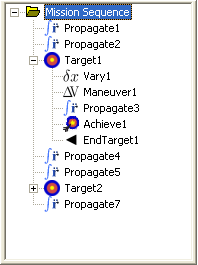
\includegraphics[99,133]{Images/HierarchicalMissionTree.png}
\caption{\label{figure:HierarchicalMissionTree}GMAT Command Sequence in the GUI}
\end{center}
\end{figure}

\textbf{Rework this piece -- it's not currently used} GMAT does not restrict the depth of the
nesting levels for the commands that control subsequences. The command classes include a counter
that monitors the current nesting level in the command sequence.  The nesting level is set when the
command is added to the linked list.  The main command sequence has a nesting level of 0.
Subsequences off of the main sequence increment the level to 1; subsequences contained in these
subsequences have a nesting level of 2, and so forth.  The subsequence termmination commands,
typically identified by an ``End'' prefix, have a nesting level set to the same level as the rest of
the subsequence, because they are the last command in the subsequence, and therefore exist at the
subsequence level.

\subsection{Command--Sandbox Interactions}

When a mission control sequence is run, all of the configured objects used in the run are copied
from the Configuration Manager into the Sandbox used for the run.  These copies are place into a
standard template library (STL) map matching the object names to pointers to the local copies in
the Sandbox.  These pointers need to be bound to the commands prior to execution of the mission
control sequence.  This late binding is performed during the initialization phase described below.
Additional details about the late bindign strategy implemented in GMAT can be found in
Section~\ref{section:SandboxLateBinding}.

During mission control sequence execution, the commands interact with the object copies to model
the interactions dictated for the model, as described in the execution section below.  These
interactions change the local copies, modeling the evolution of the system.  Once the command
sequence completes execution (either by finishing the sequence, encountering a ``Stop'' command, or
detecting a user generated stop event), each GMAT command is given the opportunity to complete any
pending operations.  This final step, described in the Finalization section below, is used to close
open file handles, clean up temporarily allocated memory, and perform any other housekeeping tasks
needed to maintain the mission control sequence for subsequent user actions.

\section{The Command Base Classes}

Figure~\ref{figure:CommandBaseClasses} shows core properties of the base classes used in the Command
subsystem.  The top level base class, GmatCommand, provides linked list interfaces and methods used
to parse command scripts.  BranchCommand adds capabilities to implement and execute commands that
run subsequences -- specifically, the Control Logic, Solver, and Function categories of commands.
Additional capabilities required by the Control Logic commands are provided by the ConditionalBranch
class.  Capabilities shared by all Solvers are implemented in the SolverBranchCommand class.

\begin{figure}
\begin{center}
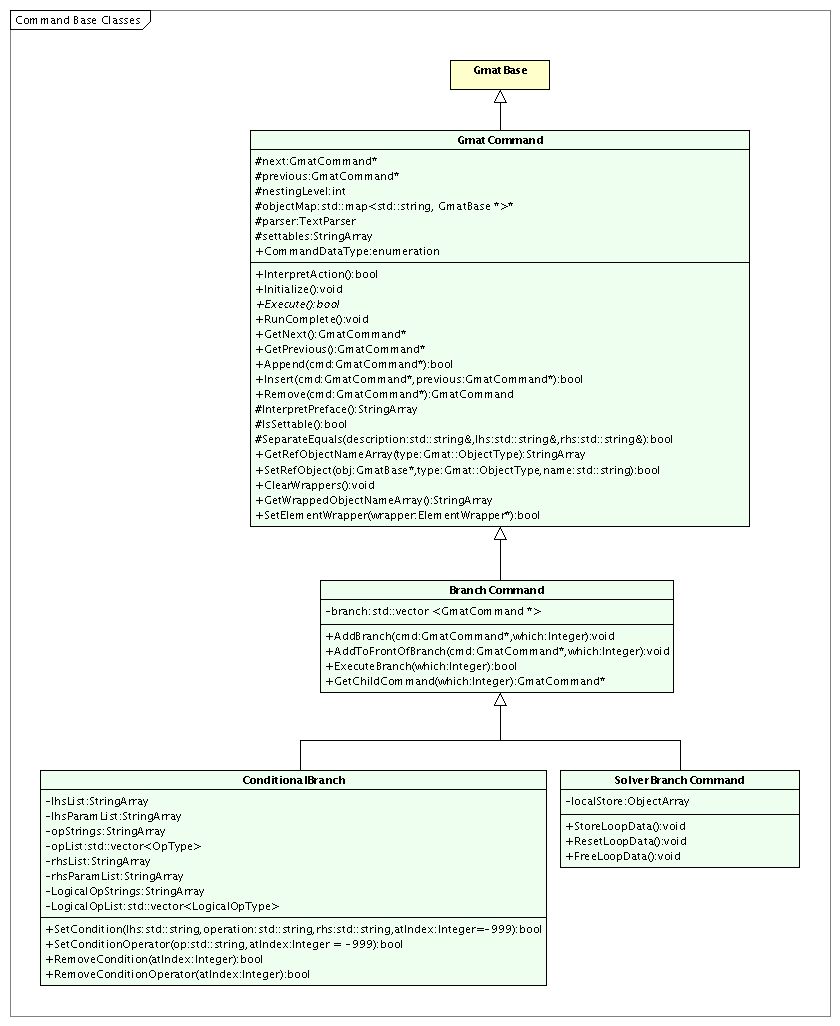
\includegraphics[405,520]{Images/CommandBaseClasses.png}
\caption{\label{figure:CommandBaseClasses}Base Classes in the Command Subsystem}
\end{center}
\end{figure}

\subsection{List Interfaces}

\textit{To be filled in}

\subsection{Object Interfaces}

\textit{To be filled in}

\subsection{Other Interfaces}

\textit{To be filled in}

\section{Script Interfaces}

The standard script syntax for a command is the command name followed by zero or more text strings
separated by white space.  Commands that are scripted using this syntax are handled generically in
the Interpreter subsystem, as described in Chapter~\ref{chapter:ScriptRW}\footnote{Some commands
that do not follow this generic description are also handled in the Interpreters at this writing.}.
Commands that use more complex scripting than a simple list of elements manage their own parsing in
a customized implementation of the InterpretAction() method.  This section describes the command
base class structures and methods that are used by commands that override InterpretAction() and
parse their configurations internally.  Parsing for Commands that do not override the
InterpretAction() method is handled in the ScriptInterpreter.  The methods described in the
following text are not used by those Commands.

\subsection{\label{section:ParametersInCommands}Data Elements in Commands}

Commands can be scripted to describe the actions taken on elements of the model (i.e. objects
instantiating GMAT classes), or to manipulate specific data elements of these objects based on the
rules encoded into the command.  When performing the latter task, the specific data element is
accessed using an ElementWrapper helper object that can manipulate data represented by the
following types: numbers, object properties, variables, array elements, and Parameter objects.  In
addition, commands may be construsted in the future that operate on Array objects and strings; the
infrastructure needed for these objects is included in the wrapper enumerations, but not yet
implemented.

The data wrappers are described in Section~\ref{section:DataWrappers}\footnote{The ElementWrappers
use the Adapter design pattern, described in \ref{section:TheAdapterPattern}}. These wrappers are
designed to be used by commands when needed to handle single valued Real data elements in the
commands.  The Gmat namespace includes an enumeration, WrapperDataType, with entries for each of the
supported data types.  This enumeration is described in Section~\ref{section:WrapperDataTypeEnum}.
The data wrappers are used to standardize the interface to numbers, object properties, variables,
array elements, and other Parameter objects to perform the command operations. Arrays and Strings
are handled separately by the commands -- arrays, because they can have more than one value, and
strings, because they do not provide Real number data for use in the commands.

\begin{figure}[htb]
\begin{center}
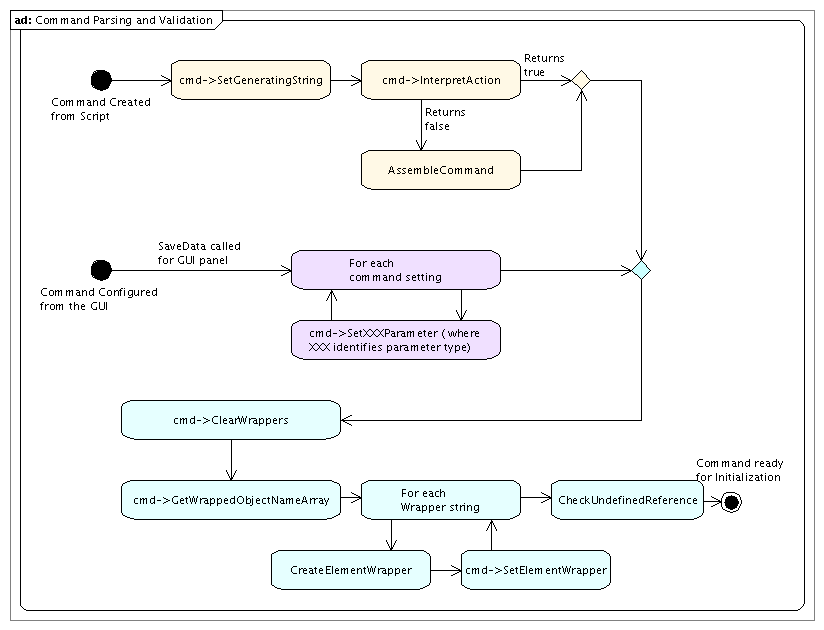
\includegraphics[412,315]{Images/CommandParsingandValidation.png}
\caption[Calls Made to Build and Validate Commands]{\label{figure:CommandParsingFlow}Calls Made in
the Interpreters to Build and Validate Commands.  Specific calls to the command are prefaced on this
diagram with the C++ pointer notation, ``cmd->''.}
\end{center}
\end{figure}

Figure~\ref{figure:CommandParsingFlow} shows an overview of the process used to build and validate
commands encountered in scripts and on the GUI.  The portions of the digram colored orange are
performed through calls launched by the ScriptInterpreter.  Commands created from the GUI follow the
procedure shown in purple.  In both cases, once the command has been built and the early binding
data has been set, the command is validated using methods provided by the Interpreter base class.
The calls made for this validation include calls that build the ElementWrapper members used in the
command.  These calls are shown in the figure in blue.

The process shown in Figure~\ref{figure:CommandParsingFlow} must be performed before the mission
control sequence can be executed in a Sandbox.  That includes identifying all of the names of
configured objects that the sequence will need, creation of any Parameters (performed in the
CheckUndefinedReference method) that will be required, and creation of the DataWrappers that will
need to be populated during Initialization in the Sandbox.

THe following subsections describe the support methods provided by the Interpreter and GUI
subsystems to configure the command objects.  These paragraphs are separated to match the three
sections of Figure~\ref{figure:CommandParsingFlow}.

\subsubsection{Scripted Command Configuration: Interpreter Support}

Scripted commands are configured using the Interpreter::CreateCommand method called from the
ScriptInterpreter while parsing a script.  The parsing process followed for commands is described
at a high level in Section~\ref{section:ParsingCommandBlocks}.  The Interpreter base class provides
several methods that facilitate that process, described here:

\begin{itemize}
\item \textbf{GmatCommand* CreateCommand(const std::string \&type, const std::string \&desc, bool
\&retFlag, GmatCommand *inCmd = NULL)}:  The method that drives the command creation process for the
ScriptInterpreter.  This method takes the generating string for the command as found in the script,
and creates an instance of the corresponding GmatCommand object.  It then calls InterpretAction() on
the command; if that call fails, it calls the Interpreter's AssembleCommand method.  Finally, it
builds any wrappers needed by the command, and validates that referenced objects used in the command
have been created.
\item \textbf{bool AssembleCommand(GmatCommand *cmd, const std::string \&desc)}:  Commands that are
not internally parsed are configured in this method.
\end{itemize}

Once this step has been completed, the command has been created and strings have been set decribing
all objects and data wrappers referenced by the command.  The data wrappers are not yet created;
thaqt process is described after the next subsection.

\subsubsection{Command Configuration in the GUI}

The GMAT GUI configures commands directly, based on the entries made by a user on the GUI panel
corresponding to the command.  Commands are created when a user inserts them into the mission
control sequence, configured with default settings.  When a user opens the configuration panel,
makes changes, and then applies the changes using either the Apply of OK button, the panel calls an
internal method, ``SaveData'', which passes the data on the panel to the command object.

The data passed into the object identifies all of teh objects referenced by the command.  Commands
configured by the GUI typically get populated with valid descriptors; as we will see shortly, the
 validation is repeated after the data wrappers are built, as described in teh next section.  All
data that requires wrappers is passed into the command as an std::string, using the
SetStringParameter method. The command stores these data for use contructing the wrappers.

\subsubsection{Interpreter Support for Wrappers and Validation}

Once GMAT has completed the steps described above, the command is configured with strings
describing wrappers and referenced objects, along with any other command specific data needed to
fully configure the command.  The final steps used configuring the command are shown in blue on
Figure~\ref{figure:CommandParsingFlow}.  These steps are all encapsulated in the Interpreter method
ValidateCommand.  The methods in the Interpreter base class used for wrapper construction and
validation are provided here:

\begin{itemize}
\item \textbf{void ValidateCommand(GmatCommand *cmd)}:  The method that executes the steps shown in
blue on the figure.  This method is called directly from the GUI, and as the final piece of
CreateCommand from the ScriptInterpreter.
\item \textbf{ElementWrapper* CreateElementWrapper(const std::string \&description)}:  This method
takes the descripion of a wrapper object and builds the corresponding wrapper.
\item \textbf{bool CheckUndefinedReference(GmatBase *obj, bool writeLine = true)}:  Method used to
verify that all referenced objects needed by the object (in this case, a Command) exist.  The
command is passed in as the first parameter.  The second parameter is a flag indicating if the line
number in the script should be written; for commands, that flag is left at its default true value.
\end{itemize}

\paragraph{CreateElementWrapper}  Of these methods, the CreateElementWrapper bears additional
explanation.  The following steps are implemented in that method:

\begin{enumerate}
\item Determine if the string is a number.  If so, create a NumberWrapper, set its value, and
return the wrapper.
\item Check to see if there a parentheses pair in the string.  If so, perform the following actions:
\begin{itemize}
\item Check to see if the text preceding the opening paren is an array.  If not, throw an exception.
\item Create an ArrayElementWrapper, and set the array name to the text preceding the opening paren.
\item Separate text enclised in the parentheses into row and column strings.
\item Call CreateElementWrapper() for the row and column strings, and set the corresponding
wrappers and strings in the ArrayElementWrapper.
\item Return the wrapper.
\end{itemize}
\item Check to see if there a period in the string.  If so, the wrapper needs to be either an
ObjectPropertyWrapper or a ParameterWrapper.  Performs these steps to create the correct type:
\begin{itemize}
\item Break apart the string using the GmatStringUtil::ParseParameter method.
\item Find the owner object, and check to see if it has the type provided in the string.  If so,
create an ObjectPropertyWrapper, otherwise create a ParameterWrapper
\item Set the description string.
\end{itemize}
Return the resulting wrapper.
\item Check to see if the string describes a Variable.  If so, create a VariableWrapper, set the
description and value, and return the wrapper; otherwise, throw an exception\footnote{A later build
will detect and return NULL for Array or String objects, so that they can be handled when needed.}.
\end{enumerate}

\subsection{Command Support for Parsing and Wrappers}

The command base class, GmatCommand, includes an instance of the TextParser described in
Section~\ref{section:TextParser}, along with an include statement for the GmatStringUtil namespace
definition (see Section~\ref{section:StringUtil} for details of the GmatStringUtil namespace).
These inclusions make all of the methods used for general purpose parsing of text from the
TextParser and the low level GmatStringUtil namespace functions available for use in command
parsing.  These elements are used by custom InterpretAction() methods when they are implemented for
the commands.

The base class also provides methods used during the creation and validation of the data wrappers.
These methods are used by the ScriptInterpreter, interacting with the Moderator in the
Interpreter::CreateCommand() method, to validate the objects required by the data wrappers.  The
methods supplied by the command base class to support data wrappers are described in
Section~\ref{section:CommandScriptingSupport}.  Before describing these methods, the wrapper
classes will be described.

\subsection{\label{section:DataWrappers}Data Type Wrapper
Classes\index{Wrappers}\index{Data Wrappers|see {Wrappers}}}

Many of the commands need to be able to treat all of the usable data types through a common
interface.  Table~\ref{table:ParameterInScriptExamples} presents representative examples to the
allowed data types in commands.  The data type interface used by the commands is captured in the
ElementWrapper class, shown with its subclasses in Figure~\ref{figure:CommandWrapperClasses}.
Derived classes are available for each of the supported types, using these classes:
NumberWrapper, ObjectPropertyWrapper, VariableWrapper, ArrayElementWrapper, and ParameterWrapper.
The Array class, when accessed as an entity rather than as a data provider for a single Real number,
is handled as a special case by any command designed to work with Array instances.  As indicated in
the table, no current command uses this capability, though it will be supported in the
NonlinearConstraint command in a future release of GMAT.  Similarly, strings are handled separately.

\begin{table}[tb]
\caption{\label{table:ParameterInScriptExamples}Script Examples of Parameters Used in Commands}
\begin{center}
\begin{tabularx}{6.3in}{|>{\raggedright\hspace{0pt}}p{1.1in}|>{\raggedright\hspace{0pt}}p{1.75in}
|X|}
\hline
\textbf{Type} & \textbf{Examples} & \textbf{Notes}
\tabularnewline \hline
Number & 1, 3.1415927, 3.986004415e5, 6.023e23 & Integers and Reals are treated identically
\tabularnewline \hline
Object Parameter & Sat.X, Burn.V, Thruster.ScaleFactor & Any object parameter
\tabularnewline \hline
Parameters & Sat.Longitude, Sat.Q4 & Any Calculated Parameter
\tabularnewline \hline
Variables & I, Var & Any Variable object
\tabularnewline \hline
Array Element & A(2,~3), B(I,~J), C(D(1,~K),~E(F(2,~3),~L)) & Any array entry.  Array row and
column indices can be specified using any allowed type
\tabularnewline \hline
Array & A & An entire array. Arrays are not yet supported in GMAT commands.  The
NonlinearConstraint command will be updated to use single column arrays (aka vectors) in a later
build.
\tabularnewline \hline
String & ``This is a string'' & A block of text treated as a single entity.
\tabularnewline \hline
\end{tabularx}
\end{center}
\end{table}

\begin{figure}[htb]
\begin{center}
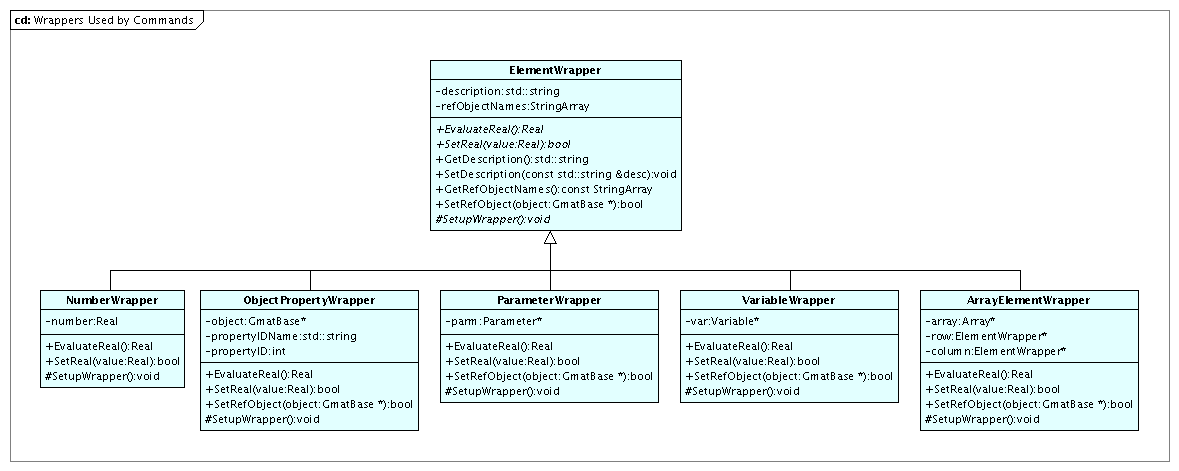
\includegraphics[460,184]{Images/WrappersUsedbyCommands.png}
\caption{\label{figure:CommandWrapperClasses}Parameter Wrappers Used by Commands}
\end{center}
\end{figure}

The wrapper classes implement the following methods:

\begin{itemize}
\item\textbf{std::string GetDescription()} Returns the current description string for the wrapper.
\item\textbf{void SetDescription(const std::string \&desc)} Sets the description string.
\item\textbf{const StringArray \&GetRefObjectNames()}: Returns a StringArray containing a list of
all reference objects used by the wrapper.
\item\textbf{bool SetRefObject(GmatBase *obj)}: Passes the a pointer to the reference object
into the wrapper so it can be assigned to the correct internal member.
\item\textbf{void SetupWrapper()}: Takes the description string and breaks it into components for
later use.
\end{itemize}

In addition, each ElementWrapper provides two abstract interfaces that can be used during command
execution:

\begin{itemize}
\item\textbf{Real EvaluateReal()} is used to calculate the current value of the wrapped
object, returning a Real number when fired.
\item\textbf{bool SetReal(const Real value)} takes a Real number as input, and sets the wrapped
element to that value.  It returns a flag indicating success or failure of the data setting
operation.
\end{itemize}

\noindent The derived wrapper classes implement these methods (and override the other methods as
needed) to access the data structures corresponding to each data type.

\subsection{\label{section:CommandScriptingSupport}Command Scripting Support Methods}

The Interpreter subsystem provides the methods needed to construct the data wrapper classes and
pass the wrappers into the commands.  GmatCommand provides the following methods to support this
process:

\begin{itemize}
\item\textbf{void ClearWrappers()}: Deletes all current wrappers in preparation for a new set of
wrapper instances.
\item\textbf{const Stringarray \&GetWrappedObjectNameArray()}: Returns a list of all wrapper
descriptions so that the required wrappers can be constructed.
\item\textbf{bool SetElementWrapper(ElementWrapper *wrapper)}: Sends the wrapper into the command.
If the wrapper is set correctly, this method returns true.  If the description contained in the
wrapper does not match a description in the command, the wrapper is destroyed, and false is returned
from this method.  All other error result in a thrown exception.
\end{itemize}

\noindent Note that commands own the wrappers passed in, and are responsible for managing the
associated memory.

\section{Executing the Sequence}

The mission control sequence is run in a GMAT Sandbox, following a series of steps described in
Section~\ref{section:SandboxMCSExecution}.  In this section, the command specific steps are
described in a bit more detail.

\subsection{Initialization}



\subsection{Execution}

\textit{To be filled in}

\subsection{Finalization}

\textit{To be filled in}

\subsection{Other Details}

\textit{To be filled in}



\chapter{Questions and Thoughts}

This chapter is for capturing questions and unaddressed issues while
we work on this document.

\begin{itemize}
     \item If a user has a measurement data file that has data for
     multiple spacecraft and multiple ground stations, how can the
     specify to only use a subset of the data.  Matt suggested using
     an Exclude field on a measurement.
\end{itemize}





\begin{thebibliography}{9}% maximum number of references (for label width)

   \bibitem{GTDS:89} Long, A., and Cappellari, J. O. \emph{et al}, ``Goddard Trajectory Determination System
    Mathematical Theory, Revision 1,"  \emph{NASA Goddard Space Flight Center}, Greenbelt, MD, 1989.

    \bibitem{DatSim:08} Long, A., \emph{et al}, ``User Guide and Mathematical Specifications for the Measurement Data Simulation Program
    Release 2.11,"  \emph{NASA Goddard Space Flight Center}, Greenbelt, MD, Sept., 2008.

\end{thebibliography}

\end{document}

%------------------------------------------------------------
%-----------------Part I:  Mathematical Specifications-------
%------------------------------------------------------------
\section{Measurement Models}

\subsection{General Form of Measurement Models}

Measurement models for orbit determination involve modelling of some
physical property of electromagnetic wave propagation and
analytically relating the computed measurement value to the
spacecraft state. \cite{GTDS:89} GMAT supports numerous measurement
models of varying complexity from simple two-way range, to GPS
carrier phase measurements.  The sections below contain the
mathematical specifications for all measurement models including
measurement corrections.  We start with ground station models
including one-way and two-way range, angles measurements, and
doppler measurements including instantaneous and integrated Doppler.

% The general form of the measurement model used by GMAT is
%%
%\begin{equation}
%   \mathcal{O}_c = f_g\left(\mathbf{r}_p^k(t^k), \dot{\mathbf{r}}_p^k(t^k),\mathbf{q}_p^k(t^k),\boldsymbol{\omega}_p^k(t^k)
%   \right) + \Delta f_{iono} + \Delta f_{tropo} + \Delta f_{rel}+ \Delta f_{abber} + \sigma_n + b
%\end{equation}
%%
%
%%
%\begin{tabbing}[htbp!]
%12345678 \= dummy line \kill
%$\mathcal{O}_c$  \>  Computed value of the measurement\\
%$\mathbf{f}_g$ \> The geometric model specific to the measurement type\\
%$\mathbf{r}_p$ \> Position of $k^{th}$ participant\\
%$\dot{\mathbf{r}}_v$ \> Velocity of $k^{th}$ participant\\
%$\mathbf{r}_o$ \> Observer position\\
%$\dot{\mathbf{r}}_o$    \> Observer velocity\\
%$t$    \> Measurement time tag\\
%$b$    \> Measurement bias\\
%$\delta a$    \> Atmospheric correction\\
%$\delta r$     \> Relativistic correction\\
%\end{tabbing}


\subsection{Range}

 \cite{DatSim:08} In both cases the range is a
measure of the distance between an observer and a vehicle.  The
geometric range is calculated using vector geometry and ignores
signal propagation times and error sources.  Most, if not all,
ground trackers provide the user with the round trip signal
propagation time.  The radiometric range model uses the best
estimate spacecraft state to determine an expected value for the
round trip signal propagation time from observer to spacecraft and
back to the observer.  Hence, the raw radiometric value is a measure
of round trip range.


\begin{equation}
    \mathcal{R}_2 = \rho^{(m,j)}_2(t_i) +c\left(b_r^{(m)}(t_i) - b_t(t_t)\right)
     + \Delta \rho_{iono}(t_i) + \Delta \rho_{tropo}(t_i)
      + \sigma_{SA} + \sigma_n + b_m
\end{equation}


\begin{tabbing}
12345678912345 \= Reynolds number based on length $s$ \kill
$\mathcal{R}_1^{(j)}$         \>  One-way pseudorange measurement from transmitting \\
$$                            \> antenna $k$ on satellite $j$ to receiving antenna $m$ on satellite $n$. \\
$\rho^{(m,j)}_1(t_i)$         \>  Geometric distance between transmitting and receiveing antenntas.\\
$b_r^{(m)}(t_i)$               \> Clock bias for receiver \\
$b_t^{(j)}(t_t)$                   \>  Clock bias for transmitter\\
$\Delta \rho^{(j)}_{iono}(t_i)$    \> Correction for ionspheric delay \\
$ \Delta \rho^{(j)}_{tropo}(t_i) $ \> Correction for  Tropospheric delay\\
$\sigma_{SA}^{(j)}$                \> Error due to selective availability \\
$\sigma_n^{(j)}$                   \> Measurement noise \\
$b_m$                              \> Measurement bias \\
$t_t$                              \> Trasmission time \\
$t_r$                              \> Receive time
\end{tabbing}


The transmission time $t_t$ and the geometric range are determined
iteratively by using fixed point iteration on the following equation
%
\begin{equation}
   t_t = t_i - \frac{\rho^{(m,j)}_1(t_i) + \Delta \rho^{(j)}_{iono}(t_i) + \Delta \rho^{(j)}_{tropo}(t_i)}{c}
\end{equation}




%
\begin{tabbing}[htbp!]
12345678 \= dummy line \kill
$\mathbf{f}_k$ \> The kinematic model specific to a measurement type\\
$\mathbf{r}_v$ \> Vehicle position\\
$\dot{\mathbf{r}}_v$ \> Vehicle velocity\\
$\mathbf{r}_o$ \> Observer position\\
$\dot{\mathbf{r}}_o$    \> Observer velocity\\
$t$    \> Measurement time tag\\
$b$    \> Measurement bias\\
$\delta a$    \> Atmospheric correction\\
$\delta r$     \> Relativistic correction\\
\end{tabbing}

The kinematic model for geometric range is simply
%
\begin{equation}
    \rho_c = \| \mathbf{r}_v(t) - \mathbf{r}_g(t)\|
\end{equation}
%

The kinematic model for radiometric two way range is
%
\begin{equation}
     \rho_c= \frac{1}{2}\left(\| \mathbf{r}_v(t_{v}) -  \mathbf{r}_g(t_{gt})  \| +
      \| \mathbf{r}_v(t_{v}) -  \mathbf{r}_g(t_{gt})  \|\right) \label{Eq:ExpectedTwoWayRange}
\end{equation}
%
where
%
\begin{tabbing}[htbp!]
12345678 \= dummy line \kill
$t_{gt}$ \> Time the uplink signal is transmitted from ground station\\
$t_{vr}$ \> Time the uplink signal is received at vehicle\\
$t_{vt}$ \> Time the downlink signal is transmitted from vehicle\\
$t_{gr}$ \> Time the downlink signal is received at ground station\\
$t_u$    \> Uplink propagation time, ( $t_{vr}$ - $t_{gt}$ )\\
$t_d$    \> Downlink propagation time, ( $t_{vt}$ - $t_{gr}$ )\\
$\rho_u$    \> Uplink distance\\
$\rho_d$    \> Downlink distance\\
$d_T$     \> Distance traveled by vehicle during transponder delay\\
$\mathbf{r}_v(t)$ \> Position of vehicle at time $t$\\
$\mathbf{r}_t(t)$ \> Position of transmitter at time $t$\\
$\mathbf{r}_r(t)$ \> Position of receiver at time $t$\\
$t$           \>  time of geometric range measurement \\
$\delta T$  \>  Vehicle's transponder delay time\\
$\delta t_a$  \>  Atmospheric delays\\
$\delta t_r$  \>  Relativistic effects\\
\end{tabbing}
%

The radiometric model is derived from the measurement geometry shown
in Fig.~\ref{Fig:RangeMeasurement}. We see that the total signal
propagation time is the sum of three times, the uplink
 signal propagation time, $t_u$, the transponder delay time, $\delta T$, and
 the downlink propagation time, $t_d$.  Hence, the observed value for signal propagation time, $t_o$, is
%
\begin{equation}
     \Delta t_o = t_{gr} - t_{gt} = t_u + \delta T + t_d
\end{equation}
%
\begin{figure}[htbp!]
    \begin{center}
    \begin{picture}(270,215)
    \special{psfile= RangeMeasurement.eps
    hscale= 75 vscale= 75 hoffset = -85 voffset = -270}
        \makebox(175,295){ $\mathbf{r}_v(t_{vr})$}
        \makebox(-25,290){ $\mathbf{r}_v(t_{vt})$}
        \makebox(85,290){ $\rho_d$}
        \makebox(-100,90){ $\mathbf{r}_g(t_{gr})$}
        \makebox(-460,90){ $\mathbf{r}_g(t_{gt})$}
        \makebox(-485,290){ $\rho_u$}
        \makebox(-305,390){ $d_T$}
    \end{picture}
    \end{center}
    \vspace{0.2 in}
    \label{Fig:RangeMeasurement}
    \caption{ Geometry of Radiometric Range Measurement}
\end{figure}
%
The elapsed time is converted to a measure of the average range
using
%
\begin{equation}
     \rho_o = \frac{c}{2}\Delta t_o
\end{equation}
%
The computed elapsed time is rigorously expressed as
%
\begin{equation}
    \Delta t_c = \frac{1}{c}\| \mathbf{r}_v(t_{vr}) -  \mathbf{r}_g(t_{gt})  \| +
    \frac{1}{c}\| \mathbf{r}_v(t_{vt}) -  \mathbf{r}_g(t_{gr})  \| + \delta T
\end{equation}
%
Assuming that the transponder delay is modelled as a measurement
bias we can write $ t_{vr} = t_{vt} = t_v$ and convert the computed
round trip time to average range:
%
\begin{equation}
     \rho_c= \frac{1}{2}\left(\| \mathbf{r}_v(t_v) -  \mathbf{r}_g(t_{gt})  \| +
      \| \mathbf{r}_v(t_v) -  \mathbf{r}_g(t_{gr})  \|\right) \label{Eq:MeasuredTwoWayRange}
\end{equation}
%
To solve Eq.~\ref{Eq:MeasuredTwoWayRange}, we must know  $t_{v}$.
For applications
 that do not require high accuracy we can approximate $t_v$ as we describe below.
  For higher fidelity applications we must solve for the uplink and downlink
  propagation times using two iterative processes.  The downlink signal propagation
  time is calculated using the following fixed point iteration on the following equation:
%
\begin{equation}
     \delta t_d^{i+1} = \frac{1}{c}\| \mathbf{r}_v( t - t_d^{i}) - \mathbf{r}_g(t)   \|
\end{equation}
%
The uplink propagation time is calculated using fixed point
iteration on
%
\begin{equation}
     \delta t_u^{i+1} = \frac{1}{c}\| \mathbf{r}_v( t - t_d) - \mathbf{r}_g(t - t_d - t_u^{i} )   \|
\end{equation}
%

\begin{eqnarray}
     \frac{\partial \rho_c (t)}{\partial \mathbf{r}_v(t_v)} &=& \frac{1}{2\rho_u\rho_d}
     \left( \rho_d(\mathbf{r}_v^T(t_v) - \mathbf{r}_T^T(t_{gt}) + \rho_u(\mathbf{r}_v^T(t_v) - \mathbf{r}_R^T(t_{gr}  ) \right)\\
     %
     \frac{\partial \rho_c (t)}{\partial \dot{\mathbf{r}}_v(t_v)} &=& \mathbf{0}_{1x3}
\end{eqnarray}

\subsection{Angles}


\end{document}
